\documentclass{sigchi}

% Use this command to override the default ACM copyright statement (e.g. for preprints). 
% Consult the conference website for the camera-ready copyright statement.


%% EXAMPLE BEGIN -- HOW TO OVERRIDE THE DEFAULT COPYRIGHT STRIP -- (July 22, 2013 - Paul Baumann)
% \toappear{Permission to make digital or hard copies of all or part of this work for personal or classroom use is 	granted without fee provided that copies are not made or distributed for profit or commercial advantage and that copies bear this notice and the full citation on the first page. Copyrights for components of this work owned by others than ACM must be honored. Abstracting with credit is permitted. To copy otherwise, or republish, to post on servers or to redistribute to lists, requires prior specific permission and/or a fee. Request permissions from permissions@acm.org. \\
% {\emph{CHI'14}}, April 26--May 1, 2014, Toronto, Canada. \\
% Copyright \copyright~2014 ACM ISBN/14/04...\$15.00. \\
% DOI string from ACM form confirmation}
%% EXAMPLE END -- HOW TO OVERRIDE THE DEFAULT COPYRIGHT STRIP -- (July 22, 2013 - Paul Baumann)


% Arabic page numbers for submission. 
% Remove this line to eliminate page numbers for the camera ready copy
% \pagenumbering{arabic}


% Load basic packages
\usepackage{balance}  % to better equalize the last page
\usepackage{graphics} % for EPS, load graphicx instead
\usepackage{times}    % comment if you want LaTeX's default font
\usepackage{url}      % llt: nicely formatted URLs
\usepackage{listings}

% llt: Define a global style for URLs, rather that the default one
\makeatletter
\def\url@leostyle{%
  \@ifundefined{selectfont}{\def\UrlFont{\sf}}{\def\UrlFont{\small\bf\ttfamily}}}
\makeatother
\urlstyle{leo}


% To make various LaTeX processors do the right thing with page size.
\def\pprw{8.5in}
\def\pprh{11in}
\special{papersize=\pprw,\pprh}
\setlength{\paperwidth}{\pprw}
\setlength{\paperheight}{\pprh}
\setlength{\pdfpagewidth}{\pprw}
\setlength{\pdfpageheight}{\pprh}

\lstdefinestyle{customc}{
  belowcaptionskip=1\baselineskip,
  breaklines=false,
  frame=M,
  xleftmargin=\parindent,
  language=JAVA,
  showstringspaces=false,
  basicstyle=\footnotesize\ttfamily,
  keywordstyle=\bfseries\color{green},
  commentstyle=\itshape\color{black},
  identifierstyle=\color{blue},
  stringstyle=\color{orange},
}

% Make sure hyperref comes last of your loaded packages, 
% to give it a fighting chance of not being over-written, 
% since its job is to redefine many LaTeX commands.
\usepackage[pdftex]{hyperref}
\hypersetup{
pdftitle={Follow-focus with Arduino},
pdfauthor={LMU Munich},
pdfkeywords={SIGCHI, proceedings, archival format},
bookmarksnumbered,
pdfstartview={FitH},
colorlinks,
citecolor=black,
filecolor=black,
linkcolor=black,
urlcolor=black,
breaklinks=true,
}

% create a shortcut to typeset table headings
\newcommand\tabhead[1]{\small\textbf{#1}}


% End of preamble. Here it comes the document.
\begin{document}

\title{Follow-focus with Arduino}

\numberofauthors{3}
\author{
  \alignauthor Christian Guerrero\\
    \affaddr{Ludwig Maximilian Universit\"at, M\"unchen, Munich, Germany}\\
    \email{christian.guerrero@campus.lmu.de}\\
  \alignauthor Arthur Moufounda\\
    \affaddr{\'{E}cole Sup\'{e}rieure Des Technologies Industrielles Avanc\'{e}es, Bidart, France}\\
    \email{a.moufounda@net.estia.fr}\\
  \alignauthor Alexander Schenker\\
    \affaddr{Ludwig Maximilian Universit\"at, M\"unchen, Munich, Germany}\\
    \email{alexander.schenker@campus.lmu.de}\\
}

\maketitle

\begin{abstract}

This paper covers the development of a novel device for focus pulling in movie production. It describes the field of application and gives an overview of established commercial and non-commercial solutions, before stating current research and deducing requirements for a new development. It further documents the challenges and solutions, that came up during the development process, before attempting a future prospect.

\end{abstract}

\keywords{
	Follow Focus; Movie Production; Remote Control; Film Set Automation; Arduino; Android;\newline
}

\section{Motivation and Background}

\subsection{General Motivation}

\subsubsection{General Description of the Topic}

In movie production, especially the part of \textit{principal photography} is considered one of the most expensive ones. This is, among other reasons, due to the often high number of scene takes, that have to be shot. \cite{kcrabb}
Usually, manual control is required in order to zoom and to keep the focus on the desired object. In classical productions, the \textit{focus puller} (or \textit{first Assistant Camera}) is a dedicated position, whose job it is to keep the focus according to the cinematographers instructions. As there is no way to correct a falsely set focus in post-production, it is considered one of the most difficult jobs on a film set. \cite{cineman}

\subsubsection{State of the Art in Follow Focus}

This section gives a brief overview of a selection of currently existing technologies in the field of follow focus. 

Andra Motion Focus is a commercial hardware system developed by Andra Motion Technologies Inc. It combines hardware-supported motion capturing with a remote controlled follow focus system. It is currently controllable optionally with an iPad or a dedicated hardware interface, called \textit{The Arc}. Andra Motion Focus is designed for portability and efficiency, in order to reduce the amount of time needed and hence the shoots' cost. Due to the high price, it aims for professional and semi-professional film-makers. \cite{andra}

The FF-X1 by PROAIM Camera is exemplary for many similar products on the market. It is a purely manual gear-driven mechanism, that is supposed to "ensure smooth accurate emphasis over your subject" \cite{proaim}. Usage is supported for a wide range of cameras. 

Lenzhound is "A super-affordable wireless follow focus system for indie filmmakers." \cite{kicklenz} It was originally featured on kickstarter by a company called Motion Dogs. The key idea of Lenzhound is, to have a simplistic, hardware- and remote-controlled Focus System. It is belt-driven and can be attached to almost any type of camera lens. Unlike Andra Motion Focus, Lenzhound addresses both amateur and independent film-makers. 

"Follow Focus" by Adi Soffer is an open source and Do-it-yourself (DIY) follow focus project from 2013. It is based on Arduino hardware and standard electronical components, which makes it relatively easy to reproduce. The source code can be found on GitHub. \cite{soffer}


\subsection{Background}

\subsubsection{Vision}

Considering the difficulties resulting from the precision required while shooting a film, and the often high number of takes, it is worth thinking about a holistic automated system. One that offers not only automated dolly shots, or remote controlled focus pulling, but one that includes everything from camera movement to image composition. As mentioned in the State of the Art section, there is a wide range of systems available. However, they are often not affordable for independent film-makers, due to their high costs. Also, for most solutions, the benefit is limited to one single use-case, such as focus pulling. 

Consequently, our vision is to create a DIY system, which combines features from several existing solutions.    


\subsubsection{Current Research at Ludwig-Maximilian-Universit\"at (LMU)}

Previous and current research conducted by LMU in Munich, Germany has come up with theoretical research on automated camera shots \cite{pburgdorf} and the development of a remote controlled camera slider \cite{pmoerwald}. 

This paper covers the prototypical development of a remote controlled focus pulling device with the long-term objective to get integrated into a system, which combines automated dolly shots, focus pulling and camera tilts.

\section{Solution}

\subsection{Our Follow Focus Approach}
Our approach is based on the ideas of \textit{DIY Follow Focus} \cite{diyff} and \textit{Soffer Follow Focus}, combined with an app-based remote control interface.

Having analyzed the existing solutions from the \textit{State of the Art} section and current research, we came up with a list of requirements, that we impose on our prototype:
\begin{itemize}
  \item The protypical device should be adaptable to a wide range of camera types. 
  \item Focus pulling should be done in realtime.
  \item The speed of focus change should be adjustable.
  \item The lense's range should be calibratable.
  \item Focus sequences should be recordable and therefore easily repeatable.
  \item The system should be controllable through an Android-based app interface.
  \item The communication between hardware and software should happen via Bluetooth Low Energy (BLE).
\end{itemize}

The adaptation to different camera types happens through an adjustable gear ring.

BLE is a low-cost wireless technology, which allows data transmission with a comparatively low energy consumption. According to the official bluetooth developer portal, it has the "ability to run for years on standard coin-cell batteries". \cite{ble}

\subsection{Methods}
To realize our aims we decided to develop an Android App for input. It sends a perpetual signal via BLE to a BLE module connected to an Arduino Nano. The Arduino processes the byte information and sends commands to a stepper driver module. The driver then controls the movement of a stepper motor. 


\subsubsection{Electrical Engineering}
Most importantly we wanted our follow focus to be portable. Therefore the elements had to be small, low energy powered and easily embeddable. These challenges had to be tackled in the planning phase of the process. So at first we had to decide between different technologies in order to meet our aims:
\begin{itemize}

\item For our requirements an Arduino Nano is more than sufficient. It is small and consumes only little.

\item For the Wireless control we use BLE for the reasons mentioned above and for compatibility reasons with other LMU projects, which use this technology as well.

\item A stepper motor works more precise and faster than a servo and has only small enertia \cite{steppervsservo}. Also with stepper we always know the exact amount of rotation we have to apply.

\item In order to link the motor to the system, we use a stepper driver. It will protect the Arduino Nano from different electrical damages that may be caused by the sudden increase of intensity by the motor. It also allows to turn in both directions.
\item The AccelStepper library for Arduino prevents the API from blocking and supports very slow speeds. Furthermore it helps to easily apply acceleration.
\item None of the electronic parts is passive. To make them all work, we need electric energy. As we also want our global system to be portable, we will use different sets of battery, because the Arduino and the step motor need to be powered separately. At least 5V and 12V respectively.
\end{itemize}
In Figures \ref{fig:Circuit} and \ref{fig:Assembly} you can see how all components are merged together into one system.

\begin{figure}
\includegraphics[width=0.4\textwidth]{circuit.png}
\caption{Circuit Diagram of the Electrical Engineering in our Follow Focus}
\label{fig:Circuit}
\end{figure}
\begin{figure}
\includegraphics[width=0.4\textwidth]{assembly.png}
\caption{Assembly Diagram of the Follow Focus System}
\label{fig:Assembly}
\end{figure}
	
\autoref{ccode} shows how the received BLE Serial data is being processed on Arduino side. The main loop always checks for connection and if so then at first we perform run() on the stepper. This will result in a step to the next position if there is one due. \\
Now there are basically two possibilities for our control. Either we use a fixed maximum speed and only change the step size or we vary the speed and use always the same step size. Our experiments showed that the second method performs more fluid and exact. So this is now how react() works: \\
the Arduino listens to incoming values \textit{0}, \textit{43}, \textit{45}, \textit{49} to \textit{57} which represent the ASCII values of the number keypad. \textit{+} adds one step to the stepper's position and \textit{-} subtracts. \textit{0} stops our stepper immediately. This is necessary as there might be some steps due, because of congestion in the output processing. With Keys \textit{1} to \textit{9} we control nine different speeds.\\
 After react() we run() again due steps and set the new due position which will be executed in the next loop.
\lstinputlisting[caption=Processing of received BLE serial data, style=customc, label={ccode}]{code.c}
 
\subsubsection{Case Modeling}
Challenges \& Solution

For building our case (see Figure \ref{fig:Case}) we faced two crucial questions: How can we achieve a small overall size to maintain portability? And which technology can we use to create a case, which is both stable and lightweight? 
We quickly realized, that premade plastic cases for electronics would be too inflexible in terms of spatial efficiency, while the quality and stability was excellent. Our first approach for a self-made case was using 3D-printing technology. First, we designed the parts with \textit{CATIA}, a 3D modeling software by \textit{Dassault Systemes} \cite{dassault}. However, the printing took a very long time and the outcome was not satisfying. Even though we expected a maximum of freedom in terms of design possibilities, the printed parts of the case turned out to be very uneven and unstable. 
Our third, and final option was the use of a laser cutter. We were able to re-utilize parts of the 3D model, which we created for the 3D-printing approach. The 3mm wooden material turned out to be ideal for our case, as it offers the needed stability, while being lightweight and easy to process. 

The finished case is composed of three compartments. The first one accommodates the electronic parts. 
A second one lies underneath and is designed exclusively for the batteries and a power button. The back of the case has two notches, which allow to open the backside easily when a battery exchange is due. In the front part of the case, there is space reserved for the stepper motor, which can be fixated with screws. The slots on the sides around the stepper motor are supposed to evacuate the heat produced by the motor when it is at work. Two holes drilled into the partition walls allow wires to connect the Arduino, stepper and battery compartments.

\begin{figure}
 	\center
 	\includegraphics[width=0.4\textwidth]{case.png}
	\caption{3D Model of our Prototype Case}
	\label{fig:Case}
\end{figure} 

\subsubsection{App Development}
Challenges

For the development the of the remote controller app, we faced various challenges. As we defined the use of BLE as one of our requirements, only a part of the available Android devices is capable of executing our application, namely those with Android 4.3 or higher and with the required hardware module built in. Currently (as of August 3, 2015), 62.1 percent of all Android devices meet the requirements software-sided, while the share of devices, which provide BLE hardware is unknown. \cite{devand} However, we do not consider this being a problem, as the advantages of BLE technology outweigh the disadvantage (compare \textit{Bluetooth Low Energy} in \textit{Our Follow Focus Approach}).

The other challenge was, how to implement the required functionalities. Here, it was important to keep the extensibility in mind. As the main goal is, to eventually embed the app and the hardware into to a larger system, it must be developed in a way, that it can be easily extended on the one hand, and that the logic can be transferred into another app on the other hand (compare \textit{Our Vision}). One of the key challenges, was the implementation of the focus sequence recording in a way, that sequences are exactly reproducible. 

Last, but not least, the User Interface (UI) should be created in a way, that makes the app easy to use, especially when it offers multiple different functionalities. As the design of a UI is not directly part of our requirements, we neglect this topic in this paper (see \autoref{fig:UI} for the prototypical UI). 

\begin{figure}
  \center
  \includegraphics[width=0.4\textwidth]{ui.png}
  \caption{Prototypical User Interface}
  \label{fig:UI}
\end{figure} 

Our Solution

As our solution for the controller, we developed an Android App for smartphones. Through the provided UI, the camera operator is able to connect to the Follow Focus device via BLE. 
Once connected, the lens range of the attached camera can be calibrated in order to prevent the stepper motor from damaging the lens focus thread.
The underlying logic for focus movement is relatively simple. The app manages two \textit{byte}-values for both speed and direction of the movement.
The speed value can be regulated via a slider element (\textit{SeekBar} in Android SDK) with a range from 0 to 100. The direction can be either right (IN), left (OUT) or neutral (no movement), and can be regulated via two buttons. The default direction is neutral, and direction changes only, while one of the two buttons is pressed.  \newline
To implement the focus sequence recording function, we had to think of a way, of how the user input could be saved including the temporal aspect. Therefore, the important information is not only \textit{what} the user does, but also \textit{when}. We basically came up with two approaches to this problem: \newline
\begin{itemize}
  \item Whenever a user input occurs, send the data and save the input type and value (e.g. speed 99), as well as the time delta from the beginning of the recording.
  \item Constantly check, save and send current speed and direction every \textit{x} milliseconds.
\end{itemize}

As one of the key aspects of recording a sequence is reliable repeatability, we figured that the second option would offer the better results (in terms of result stability). Due to expected latency on both the master's side (i.e. the mobile android device) and the slave (the follow focus device), we expect the first option to lead to irregular playback result. \newline
The sampling approach of the second option offers regular samples, which can be iterated through in the defined interval in order to exactly repeat the original input.

\lstinputlisting[caption=Focus Sequence Sampling, style=customc, label={javacode}]{code.java}

As can be seen in \autoref{javacode}, a timer thread in the controller app executes a function every \textit{EXECUTION\_INTERVAL} miliseconds. We defined this as an integer constant with the value of 50, which turned out to deliver the most stable results in our tests. 

The calibration works in the following way: The user can move the cameras' focus ring via the \textit{IN} and \textit{OUT} buttons to either the minimum or the maximum stop. By pressing the \textit{set min}, respective \textit{set max} button, the app sends a signal to the Arduino. Upon arrival, it responds with the current position of the stepper motor. The minimum and maximum positions are saved in variables throughout the session. Knowing the current speed and direction, the app also knows the position of the stepper motor at all times. Hence, it can prohibit movement past the limits of the lens.

\begin{figure}
  \center
  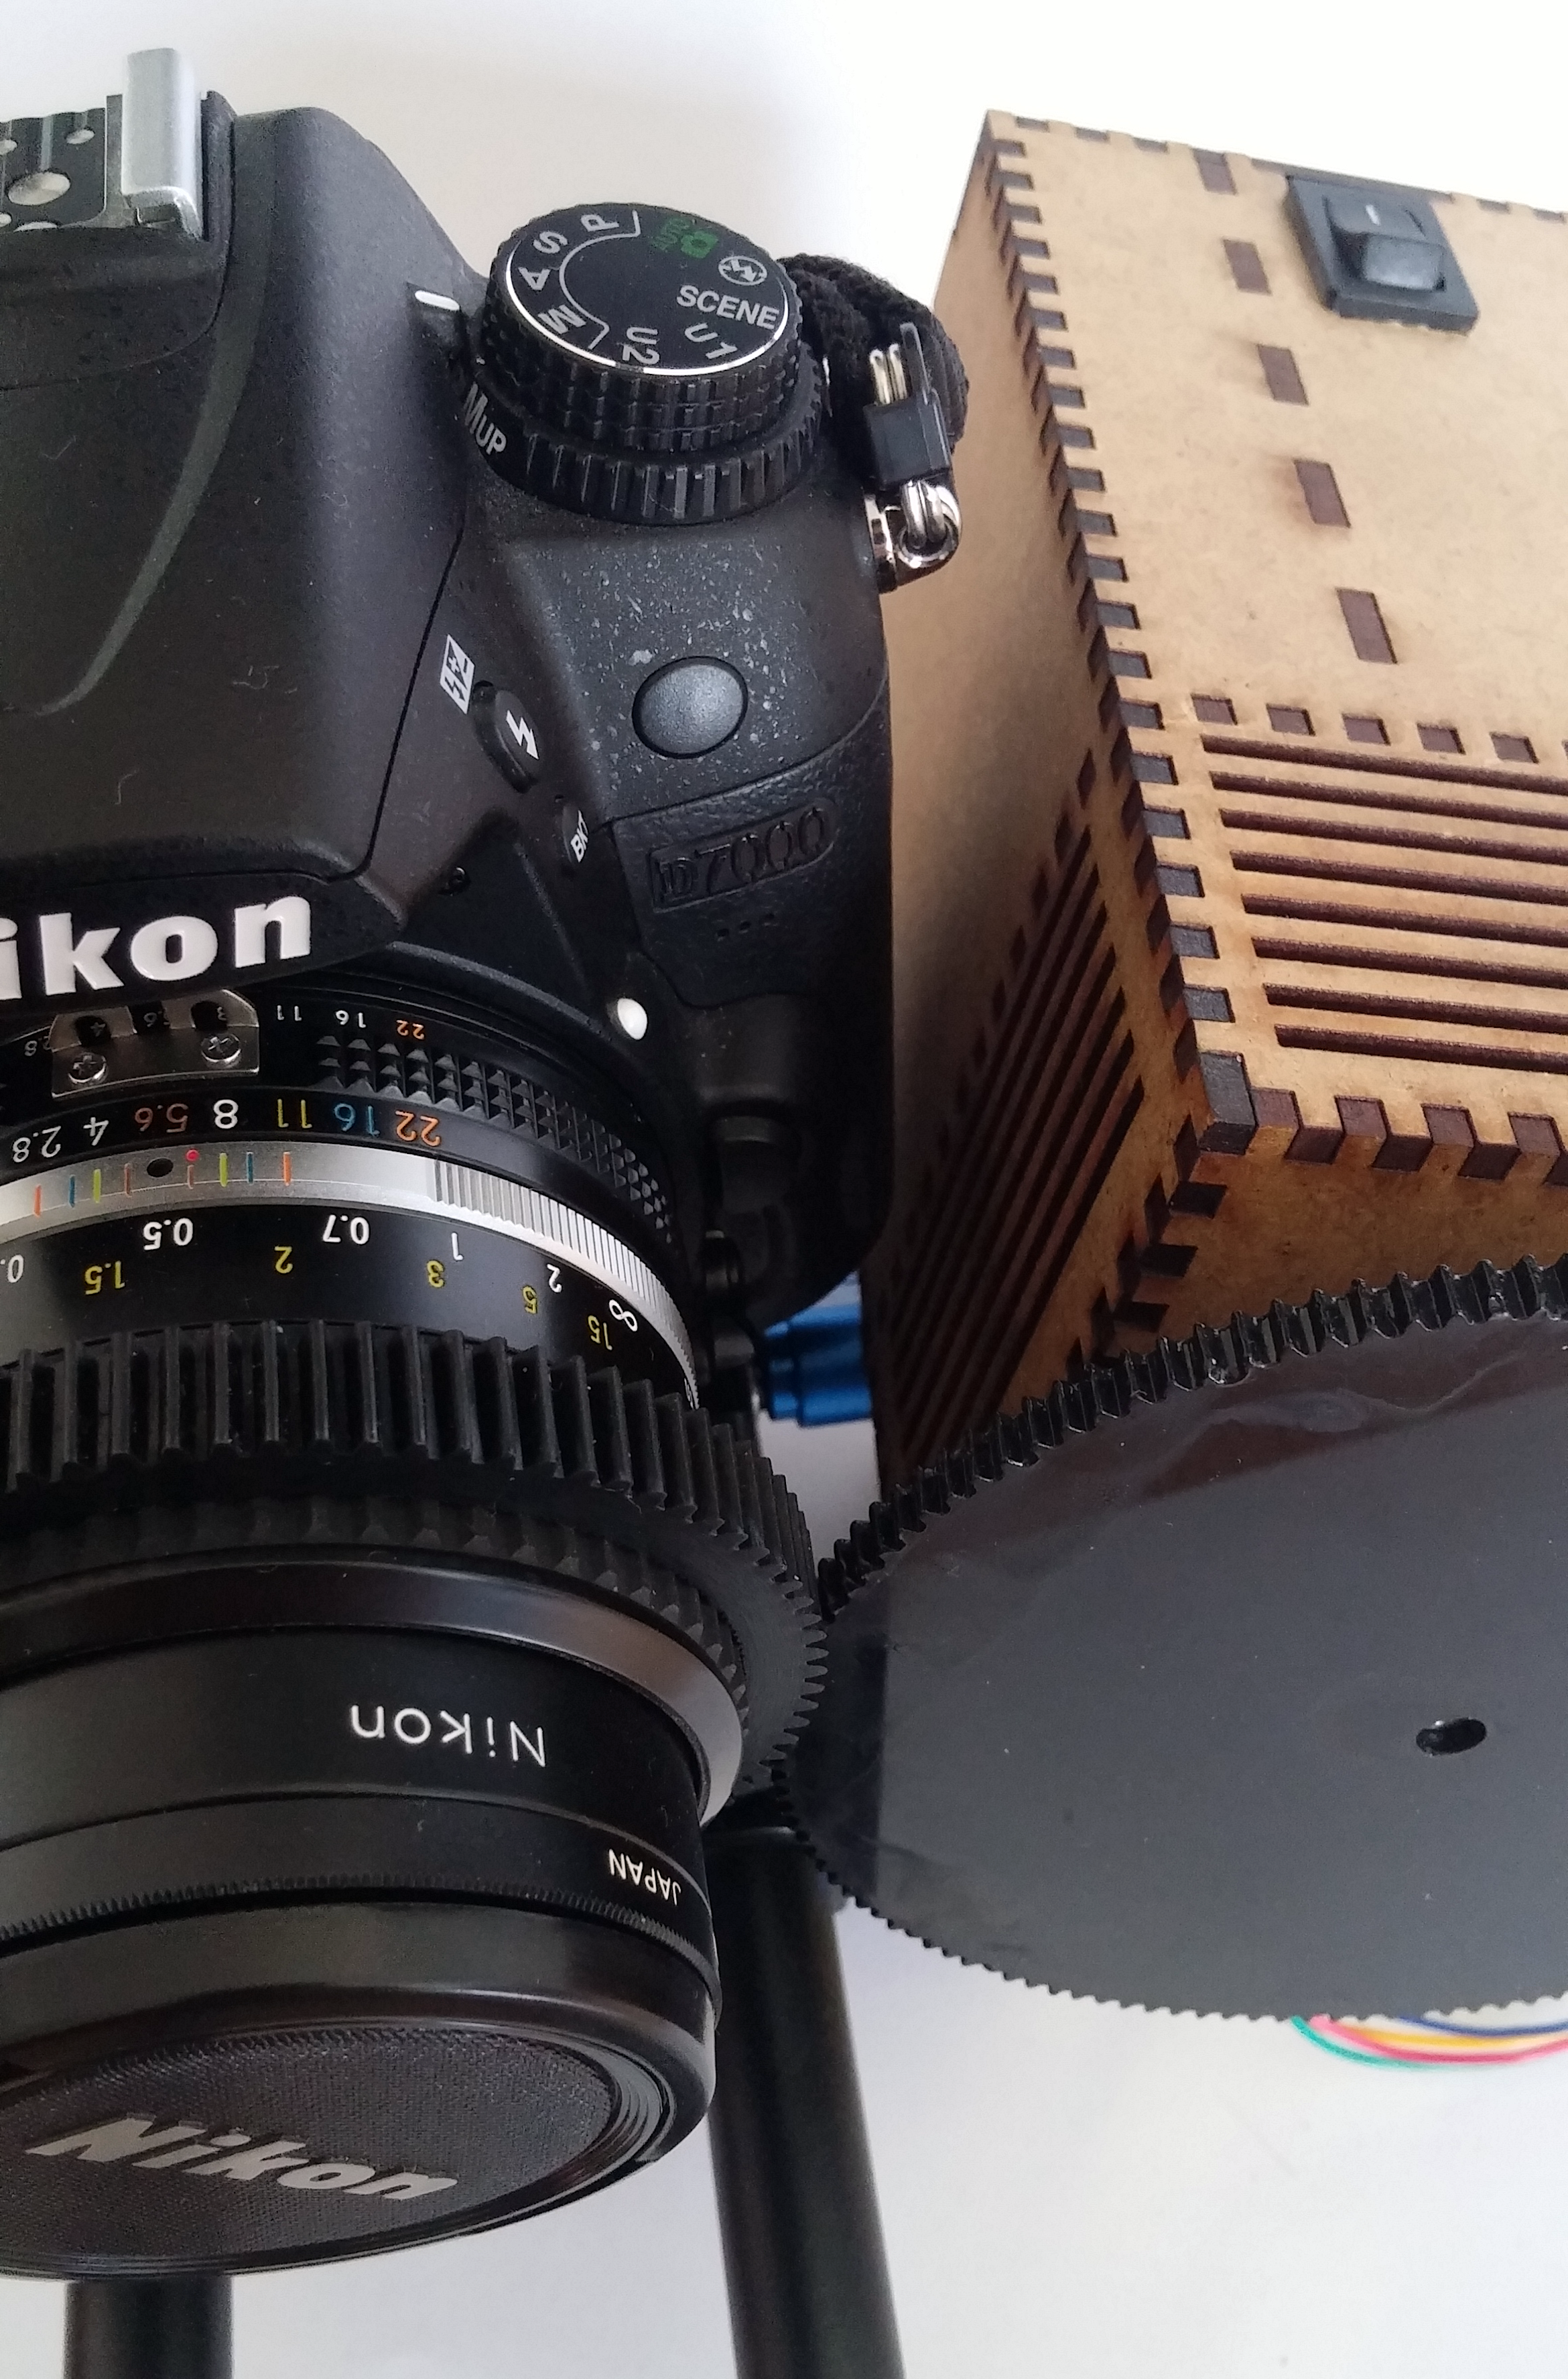
\includegraphics[width=0.4\textwidth]{prototype.png}
  \caption{Assembled Prototype}
  \label{fig:prototype}
\end{figure} 

\section{Discussion \& Next Steps}

Regarding the existence of other DIY projects, one might come up with the question \textit{Why is this important?} Admittedly, the current state is not much more than a combination and extension of the named. Though, we believe that the real strength of this project lies in its technological and topical compatibility with current research projects at LMU. Having the vision of a system in mind, that remotely controls all matters of a camera operator via an Android app, this paper covers a necessary and logical step towards the big picture. 
However, there are things that have to be addressed up front: 
\begin{itemize}
  \item The UI of our controller app is rather provisorily. Even though we deliberately neglected this topic in the scope of this paper, it is a major point for a good usability within a complex control environment.
  \item Vernier adjustment of the mechanical parts. The size of the gear and the gear transmission ratio have to be tested under real circumstances, in order to make sure that the movement suits the needs of a film production scenario.
  \item The same applies to the parameters in the Arduino software. Step size and movement speed have to be adjusted to ensure smooth movements throughout a focus sequence.
\end{itemize}

The case is equipped with its own power supply, as well as braces, that allow attachment to a camera rail. That means, that the current system can be integrated into the existing camera slider (compare \textit{Current Research at LMU}) independently, from a hardware perspective. 

Software-sided, the next step would be to conceptualize and develop a mobile application, that controls and records not only focus sequences, but also many different aspects of the camera operator related tasks. This is why the outcome of our follow focus app should be seen more as a proof of concept, rather than a fully matured product.

\autoref{fig:prototype} shows the assembled prototype together with a DSLR Camera.

\section{Conclusion}

Conclusively, this work has shown, that a more advanced tool for focus pulling can be developed with relatively simple means. The availability of existing open source projects, such as Soffer Follow Focus \cite{soffer} or DIY Follow Focus \cite{diyff}, as well as fairly low priced electronic components lay the foundation for many DIY opportunities. Advanced commercial projects like Andra Motion Focus \cite{andra} represent the current state of the art, and, with their multitude of novel features, serve as a source of inspiration for own projects.

\balance

\bibliographystyle{acm-sigchi}
\bibliography{sample}
\end{document}
